\documentclass[article]{jss}

%% -- Set-up document -------------------------------------------------------------
%%
%%
%%
%%

%% -- LaTeX packages and custom commands ---------------------------------------

%% recommended packages
\usepackage{thumbpdf,lmodern}

%% more packages 
\usepackage{multirow, amsmath, tikz} % for table, equations, and flow chart figure (respectively)
\usetikzlibrary{fit, positioning} % for flow chart figure

%% new custom commands
\newcommand{\class}[1]{`\code{#1}'}
\newcommand{\fct}[1]{\code{#1()}}

%% For Sweave-based articles about R packages:
%% need no \usepackage{Sweave}



%% -- Article metainformation (author, title, ...) -----------------------------

%% - \author{} with primary affiliation
%% - \Plainauthor{} without affiliations
%% - Separate authors by \And or \AND (in \author) or by comma (in \Plainauthor).
%% - \AND starts a new line, \And does not.
\author{Hanne Oberman\\Utrecht University \AND \\ Research Report (Preparation for Research Master Thesis, Research Seminar) \\ Methodology and Statistics for the Behavioural, Biomedical and Social Sciences}
   % \And Second Author\\Plus Affiliation}
\Plainauthor{Hanne Oberman}

%% - \title{} in title case
%% - \Plaintitle{} without LaTeX markup (if any)
%% - \Shorttitle{} with LaTeX markup (if any), used as running title
\title{A Note on Convergence Diagnostics for Multiple Imputation Algorithms}
\Plaintitle{A Note on Convergence Diagnostics for Multiple Imputation Algorithms}
\Shorttitle{Convergence Diagnostics for MI}

%% - \Abstract{} almost as usual
\Abstract{
This note investigates how algorithmic convergence of multiple imputation procedures---methodology to circumvent the ubiquitous problem of missing data---may be diagnosed. We conclude that potential scale reduction factor $\widehat{R}$ and autocorrelation may be appropriate convergence diagnostics, but their performance differs from conventional applications to iterative algorithmic procedures. These results will be implemented into an interactive framework for the evaluation of multiple imputation methods that is under development as Research Master's thesis.}

%% - \Keywords{} with LaTeX markup, at least one required
%% - \Plainkeywords{} without LaTeX markup (if necessary)
%% - Should be comma-separated and in sentence case.
\Keywords{multiple imputation, convergence, mice, \proglang{R}}
\Plainkeywords{multiple imputation, convergence, mice, R}

%% - \Address{} of at least one author
%% - May contain multiple affiliations for each author
%%   (in extra lines, separated by \emph{and}\\).
%% - May contain multiple authors for the same affiliation
%%   (in the same first line, separated by comma).
\Address{
  Hanne Ida Oberman, BSc.\\
  Methodology and Statistics for the Behavioural, Biomedical and Social Sciences\\
  Department of Methodology and Statistics\\
  Faculty of Social and Behavioral Sciences\\
  Utrecht University\\
  Heidelberglaan~15, 3500 Utrecht, The Netherlands\\
  E-mail: \email{h.i.oberman@uu.nl} % \\
  URL: \url{https://hanneoberman.github.io/}
}

\begin{document}


%% -- Introduction -------------------------------------------------------------
%%
%%
%%
%%

\section{Introduction} \label{sec:intro} 

At some point, any scientist conducting statistical analyses will run into a missing data problem \citep{alli02}. Missingness is problematic because statistical inference cannot be performed on incomplete data without employing \emph{ad hoc} solutions (e.g., list-wise deletion), which may yield wildly invalid results \citep{buur18}. A popular answer to the ubiquitous problem of missing information is to use the framework of multiple imputation (MI), proposed by \cite{rubin87}. MI is an iterative algorithmic procedure in which missing datapoints are `imputed' (i.e. filled in) several times. The variability between imputations is used to reflect how much uncertainty in the inference is introduced by the missingness. Therefore, MI can provide valid inferences despite missing information. 

To obtain valid inferences with MI, the variability between imputations should be properly represented \citep{rubin87, buur18}. If this variability is under-estimated, confidence intervals around estimates will be too narrow, which can yield spurious results. Over-estimation of the variance between imputations results in unnecessarily wide confidence intervals, which can be costly because it lowers the statistical power. Since both of these situations are undesirable, imputations and their variability should be evaluated. Evaluation measures, however, are currently missing or under-developed in MI software, like the world-leading \pkg{mice} package \citep{mice} in \proglang{R} \citep{R}. 
The goal of this research project is to develop novel methodology and guidelines for evaluating MI methods. These tools will subsequently be implemented in an interactive evaluation framework for multiple imputation, which will aid applied researchers in drawing valid inference from incomplete datasets. 

This note provides the theoretical foundation towards the diagnostic evaluation of %the convergence of 
multiple imputation algorithms. For reasons of brevity, we only focus on the MI algorithm implemented in \pkg{mice} \citep{mice}. 
The convergence properties of this MI algorithm are investigated through model-based simulation\footnotemark.%The results of this simulation study are guidelines for assessing convergence of MI algorithms. These guidelines will be implemented in an interactive evaluation tool for \pkg{mice}, `ShinyMICE', which is currently under development. 
\footnotetext{All programming code used in this note is available from \href{https://github.com/gerkovink/shinyMice/simulation}{github.com/gerkovink/ShinyMICE/simulation}.} 
We will evaluate how convergence of the MI algorithm can be diagnosed.

%% -- Terminology ---------------------------------------------------------------
\subsection{Terminology} \label{sec:terms}

%The intended audience of this note consists of anyone who uses multiple imputation to solve missing data problem. 
This note follows notation and conventions of \pkg{mice} \citep{mice}. % to suit the \pkg{mice} environment, see \cite[p.~4]{mice}. %Deviations from the `original' notation by \cite{rubin87} are described in \citep[\S~2.2.3]{buur18}.
Basic familiarity with MI methodology is assumed.\footnote{For the theoretical foundation of MI, see \cite{rubin87}. For an accessible and comprehensive introduction to MI from an applied perspective, see e.g. \cite{buur18}.} 

Let $Y$ denote an $n \times p$ matrix containing the data values on $p$ variables for all $n$ units in a sample. The collection of observed data values in $Y$ is denoted by $Y_{obs}$, and will be referred to as `incomplete' or `observed' data. The missing part of $Y$ is denoted by $Y_{mis}$. Which parts of $Y$ are missing is determined by the `missingness mechanism'.  
This note only considers a `missing completely at random' (MCAR) mechanism, where the probability of being missing is equal for all $n \times p$ cells in $Y$ \citep{rubin87}.

Figure \ref{fig:steps} provides an overview of the steps involved with MI---from incomplete data, to $m$ completed datasets, to $m$ estimated quantities of interest ($\hat{Q}$s), to a single pooled estimate $\bar{Q}$.
This note focuses on the algorithmic properties of the imputation step. 

The MI algorithm in \pkg{mice} has an iterative nature. For each missing datapoint in $Y_{mis}$, $m$ `chains' of potential values are sampled. Only the ultimate sample that each chain lands on is imputed. The number of iterations per chain will be denoted with $T$, where $t$ varies over the integers $1, 2, \dots, T$.  %This is repeated $m$ times. Imputed values are the ultimate samples of a `chain' of For each imputed value ($t = T$), a s for each missing datapoint in $Y_{mis}$, . Each of the $m$ chains starts with an initial value, drawn randomly from $Y_{obs}$. The chains are terminated after a predefined number of iterations. , and subsequently used in the analysis and pooling steps. 
The collection of samples between the initial value (at $t=1$) and the imputed value (at $t=T$) will be referred to as an `imputation chain'. 

\begin{figure}
\label{fig:steps}
\centering
	\large{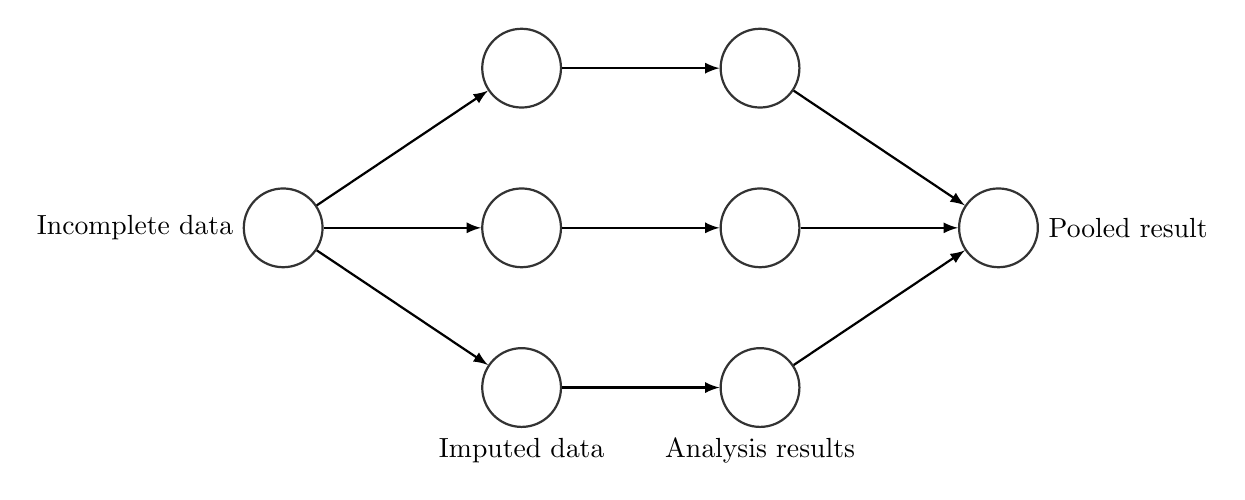
\begin{tikzpicture}
	\tikzstyle{main}=[circle, minimum size = 10mm, thick, draw =black!80, node distance = 20mm]
\tikzstyle{connect}=[-latex, thick]
\node[main, fill = white!100] (data) [label=left:Incomplete data] { };
\node[main] (mids) [right=of data] { };
\node[main] (mids2) [above=10mm of mids] { };
\node[main] (mids3) [below=10mm of mids,label=below:Imputed data] { };
\node[main] (mira) [right=of mids] {};
\node[main] (mira2) [above=10mm of mira] { };
\node[main] (mira3) [below=10mm of mira,label=below:Analysis results] { };
\node[main, fill = white!100] (mipo) [right=of mira,label=right:Pooled result] { };
\path (data) edge [connect] (mids)
      (data) edge [connect] (mids2)
      (data) edge [connect] (mids3)
      (mids) edge [connect] (mira)
      (mids2) edge [connect] (mira2)
      (mids3) edge [connect] (mira3)
		  (mira) edge [connect] (mipo)
		  (mira2) edge [connect] (mipo)
		  (mira3) edge [connect] (mipo);
\end{tikzpicture}}
\caption{Scheme of the main steps in multiple imputation \citep[$m = 3$; adapted from][\S~1.4.1]{buur18}. {\footnotesize Missing data in dataset $Y$ is `imputed' (i.e., filled in) $m$ times. The imputed data is combined with the observed data ($Y_{obs}$) to create $m$ completed datasets. On each completed dataset, the analysis of scientific interest (or `substantive model') is performed. The quantity of scientific interest (e.g., a regression coefficient) is denoted with $Q$. Since $Q$ is estimated on each completed dataset, $m$ separate $\hat{Q}$-values are obtained. These $m$ values are combined into a single pooled estimate $\bar{Q}$.}} 
\end{figure}

\begin{figure}
%\label{fig:steps2}
\centering
	\large{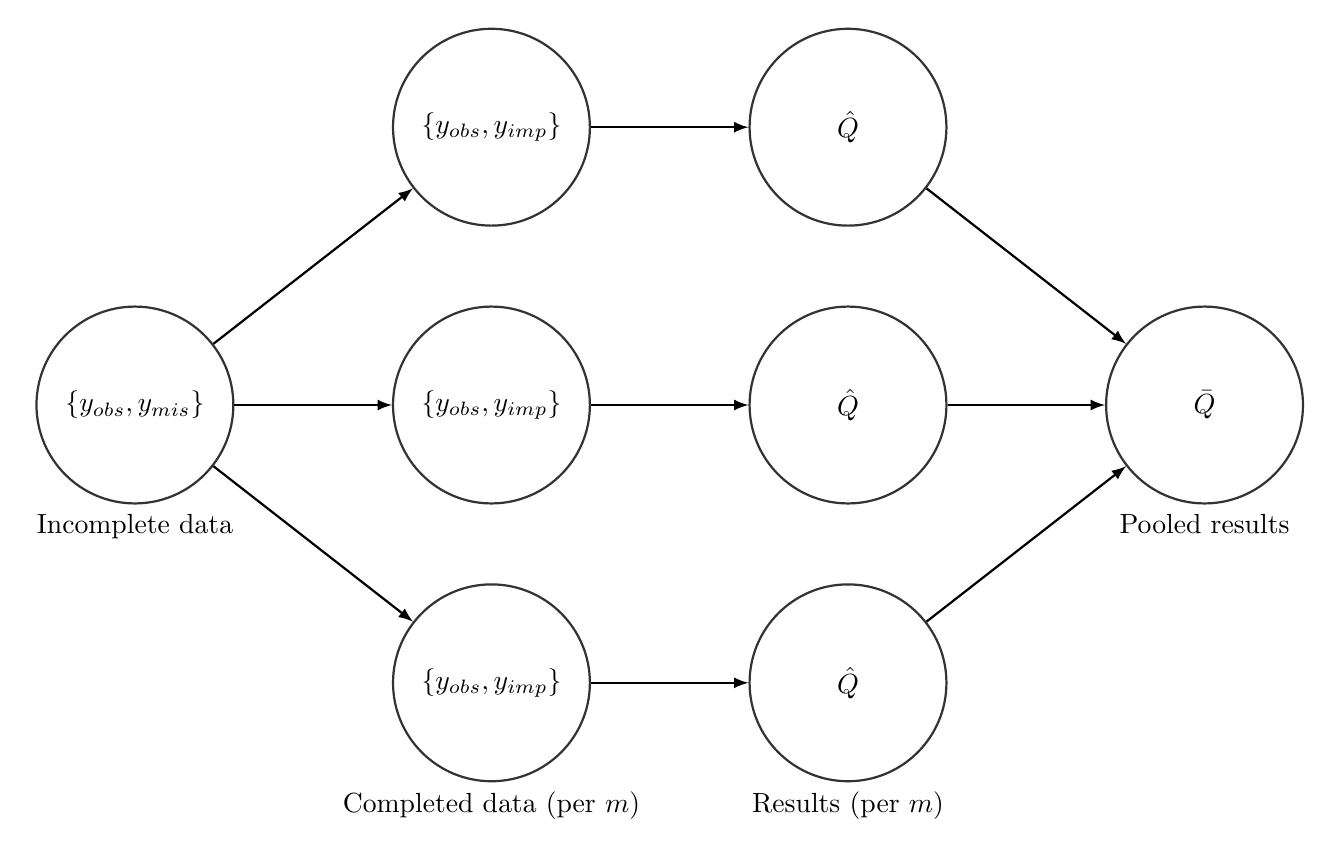
\begin{tikzpicture}
	\tikzstyle{main}=[circle, minimum size = 25mm, thick, draw =black!80, node distance = 20mm]
\tikzstyle{connect}=[-latex, thick]
\node[main, fill = white!100] (data) [label=below:Incomplete data] {$\{y_{obs}, y_{mis}\}$};
\node[main] (mids) [right=of data] { $\{y_{obs}, y_{imp}\}$};
\node[main] (mids2) [above=10mm of mids] {$\{y_{obs}, y_{imp}\}$ };
\node[main] (mids3) [below=10mm of mids,label=below: Completed data (per $m$)] { $\{y_{obs}, y_{imp}\}$};
\node[main] (mira) [right=of mids] {$\hat{Q}$};
\node[main] (mira2) [above=10mm of mira] {$\hat{Q}$ };
\node[main] (mira3) [below=10mm of mira,label=below: Results (per $m$)] {$\hat{Q}$ };
\node[main, fill = white!100] (mipo) [right=of mira,label=below:Pooled results] {$\bar{Q}$ };
\path (data) edge [connect] (mids)
      (data) edge [connect] (mids2)
      (data) edge [connect] (mids3)
      (mids) edge [connect] (mira)
      (mids2) edge [connect] (mira2)
      (mids3) edge [connect] (mira3)
		  (mira) edge [connect] (mipo)
		  (mira2) edge [connect] (mipo)
		  (mira3) edge [connect] (mipo);
\end{tikzpicture}}
%\caption{Scheme of the main steps in multiple imputation \citep[$m = 3$; adapted from][\S~1.4.1]{buur18}. {\footnotesize Missing data in dataset $Y$ is `imputed' (i.e., filled in) $m$ times. The imputed data is combined with the observed data ($Y_{obs}$) to create $m$ completed datasets. On each completed dataset, the analysis of scientific interest (or `substantive model') is performed. The quantity of scientific interest (e.g., a regression coefficient) is denoted with $Q$. Since $Q$ is estimated on each completed dataset, $m$ separate $\hat{Q}$-values are obtained. These $m$ values are combined into a single pooled estimate $\bar{Q}$. $\{y_{obs}, y_{mis}\}$ }} 
\end{figure}

%% -- Theoretical Background ---------------------------------------------------------------
\subsection{Theoretical Background} \label{sec:background}

There is no scientific consensus on the convergence properties of multiple imputation algorithms \citep{taka17}. Some default techniques in \pkg{mice} might not yield converged states at all \citep{murr18}. Therefore, algorithmic convergence should be monitored carefully. The diagnostic evaluation of convergence is preferred over the current practice---visually inspecting imputation chains for signs of non-convergence---since the latter may be challenging to the untrained eye \citep[\S~6.5.2]{buur18}. 

The application of convergence diagnostics to MI methods has not been systematically studied \citep{buur18}. The measures that are available for diagnosing convergence of iterative algorithmic procedures (Markov chain Monte Carlo methods; e.g., \pkg{mice} algorithms or Gibbs samplers) generally evaluate signs of non-convergence \citep{hoff09}. Non-convergence may be present as non-stationarity within chains (i.e., trending), or as slow mixing between chains (i.e., no intermingling). 
% Most convergence diagnostics target either of the two components. The stationarity component of convergence may be evaluated with autocorrelation \citep[$AC$; ][]{scha97, gelm13}, numeric standard error \citep[or `MC error'; ][]{gewe92}, and Raftery and Lewis's (\citeyear{raft91}) procedure to determine the effect of trending within chains. 
%\footnote{All of these methods evaluate the convergence of univariate scalar summaries (e.g., chain means or variances). These convergence diagnostics cannot diagnose convergence of multivariable statistics (i.e., relations between scalar summaries). \cite{buur18} proposed to implement multivariable evaluation through eigenvalue decomposition \cite{mack03}. This method is outside of the scope of the current study.}%  he eigenvector decomposition method proposed by McKay \citep{mcka03}.} 
% The mixing component can be assessed with the potential scale reduction factor $\widehat{R}$ \citep[a.k.a. `Gelman-Rubin statistic';][]{gelm92}. With an adapted version of $\widehat{R}$, proposed by \cite{veht19}, we might also evaluate the stationarity component of convergence. This would make $\widehat{R}$ a general convergence diagnostic. The application of $\widehat{R}$ to assess stationarity has not been thoroughly investigated. Therefore, this study employs both $\widehat{R}$ and autocorrelation to investigate convergence, as recommended by \cite[p.~898]{cowl96}.
The mixing component of convergence may be evaluated with the potential scale reduction factor, $\widehat{R}$ \citep[a.k.a. `Gelman-Rubin statistic';][]{gelm92}\footnotemark. The stationarity component may be assessed through autocorrelations. Other convergence diagnostics are outside of the scope of this study.

\footnotetext{An adapted version of $\widehat{R}$ might also be used to diagnose non-stationarity.}

To define $\widehat{R}$, we follow notation by \cite[p.~5]{veht19}. Let $M$ be the total number of chains, $T$ the number of iterations per chain, and $\theta$ the scalar summary of interest (e.g., chain mean or chain variance). For each chain ($m = 1, 2, \dots, M$), we estimate the variance of $\theta$, and average these to obtain within-chain variance $W$.

\begin{align*}
W&=\frac{1}{M} \sum_{m=1}^{M} s_{j}^{2},  \text { where } s_{m}^{2}=\frac{1}{T-1} \sum_{t=1}^{T}\left(\theta^{(t m)}-\bar{\theta}^{(\cdot m)}\right)^{2}. %\text{ \cite[p.~5]{veht19}} 
\end{align*}

We then estimate between-chain variance $B$ as the variance of the collection of average $\theta$ per chain.

\begin{align*}
B&=\frac{T}{M-1} \sum_{m=1}^{M}\left(\bar{\theta}^{(\cdot m)}-\bar{\theta}^{(\cdot \cdot)}\right)^{2}, \text { where } \bar{\theta}^{(\cdot m)}=\frac{1}{T} \sum_{t=1}^{T} \theta^{(t m)}, \quad \bar{\theta}^{(\cdot \cdot)}=\frac{1}{M} \sum_{m=1}^{M} \bar{\theta}^{(\cdot m)} \\
 %\text{ \cite[p.~5]{veht19}} 
\end{align*}

From the between- and within-chain variances we compute a weighted average, $\widehat{\operatorname{var}}^{+}$, which over-estimates the total variance of $\theta$. $\widehat{R}$ is then obtained as a ratio between the over-estimated total variance and the within-chain variance:

\begin{equation*}
\widehat{R}=\sqrt{\frac{\widehat{\operatorname{var}}^{+}(\theta | y)}{W}},
\text{ where } \widehat{\operatorname{var}}^{+}(\theta | y)=\frac{N-1}{N} W+\frac{1}{N} B.
\end{equation*}

We can interpret $\widehat{R}$ as potential scale reduction factor since it indicates by how much the variance of $\theta$ could be shrunken down if an infinite number of iterations per chain would be run \citep{gelm92}. This interpretation assumes that chains are `over-dispersed' at $t=1$, and reach convergence as $T \to \infty$. Over-dispersion implies that the initial values of the chains are `far away' from the target distribution and each other. When all chains sample independent of their initial values, the mixing component of convergence is satisfied, and $\widehat{R}$-values will be close to one. High $\widehat{R}$-values thus indicate non-convergence. The conventionally acceptable threshold for convergence was $\widehat{R} < 1.2$ \citep{gelm92}. More recently, \cite{veht19} proposed a more stringent threshold of $\widehat{R} < 1.01$. 

Following the same notation, we define autocorrelation as the correlation between two subsequent $\theta$-values within the same chain\footnotemark  \citep[p.~147]{lync07}. %. 
%
\begin{equation*}
AC = \left( \frac{T}{T-1} \right) \frac{\sum_{t=1}^{T-1}(\theta_t - \bar{\theta}^{(\cdot m)})(\theta_{t+1} - \bar{\theta}^{(\cdot m)})}{\sum_{t=1}^{T}(\theta_t - \bar{\theta}^{(\cdot m)})^2}.
\end{equation*}
%
\footnotetext{In this study we only consider $AC$ at lag 1, i.e., the correlation between the $t^{th}$ and $t+1^{th}$ iteration of the same chain.}

We can interpret $AC$-values as a measure of stationarity. If $AC$-values are close to zero, there is no dependence between subsequent samples within imputation chains. Positive $AC$-values, however, indicate recurrence. If $\theta$-values of subsequent iterations are similar, trending may occur. Negative $AC$-values show no threat to the stationarity component of convergence. On the contrary even---negative $AC$-values indicate that $\theta$-values of subsequent iterations diverge from one-another, which may increase the variance of $\theta$ and speed up convergence. As convergence diagnostic, the interest is therefore in positive $AC$-values. 
\footnote{Moreover, the magnitude of $AC$-values may be evaluated statistically, but that is outside of this note's scope.}

In short, convergence is reached when there is no dependency between subsequent iterations of imputation chains ($AC = 0$), and chains intermingle such that the only difference between the chains is caused by the randomness induced by the algorithm ($\widehat{R} = 1$).

%% -- Hypothesis -------------------------------------------------------------
\subsection{Simulation Hypothesis} \label{sec:hypothesis}

This study evaluates whether $\widehat{R}$ and $AC$ could diagnose convergence of multiple imputation algorithms. We assess the performance of the two convergence diagnostics against the recommended evaluation criteria for MI methods \citep[i.e., average bias, average confidence interval width, and empirical coverage rate across simulations;][\S~2.5.2]{buur18}. %That is, there is no baseline measure available to evaluate performance against.The current practice of visually inspecting imputation chains for signs of non-mixing or non-stationarity can only diagnose severely pathological cases of non-convergence. %\footnote{We could also look at distributional characteristics, and plausibility of imputed values, see \cite{vinknd} (n.d.). For now, this is outside of the scope of this study.} 
Based on an empirical finding \citep{lace07}, we hypothesize that $\widehat{R}$ will over-estimate non-convergence of MI algorithms. The threshold of $\widehat{R} < 1.01$ will then be too stringent for diagnosing convergence. This over-estimation may, however, be diminished because $\widehat{R}$ can falsely diagnose convergence if initial values of the algorithm are not appropriately over-dispersed \cite[p~437]{broo98}. In \pkg{mice}, initial values are chosen randomly from the observed data. Therefore, we cannot be certain that the initial values are over-dispersed. We expect this to have little effect on the hypothesized performance of $\widehat{R}$. No hypothesis was formulated about the performance of $AC$ as convergence diagnostic.


%% -- Methods ---------------------------------------------------------------
%%
%%
%%
%%

\section{Methods} \label{sec:methods}

We use model-based simulation in \proglang{R} to perform multiple imputation under 100 simulation conditions. In each condition, the MI algorithm comprises of a different imputation chain length ($T = 1, 2, \dots, 100$). The number of simulation runs per condition is 1000. For each simulation condition (i.e., number of iterations) and each repetition (i.e., simulation run) we compute convergence diagnostics ($\widehat{R}$ and autocorrelation) and simulation diagnostics (bias, confidence interval width and coverage). These diagnostics are aggregated across repetitions to obtain their average value per simulation condition.
The simulation set-up is summarized in the pseudo-code below.\footnote{The complete \proglang{R} script of the simulation study is available from \href{https://github.com/gerkovink/shinyMice/simulation}{github.com/gerkovink/ShinyMICE/simulation}.}

\begin{Code}
# pseudo-code of simulation 
simulate data 
for (number of simulation runs from 1 to 1000)
  for (number of iterations from 1 to 100)
    create missingness
    impute the missingness
    compute convergence diagnostics
    perform analysis
    pool results
    compute simulation diagnostics
aggregate convergence and simulation diagnostics
\end{Code}

%% -- Data -------------------------------------------------------------
\subsection{Data simulation}

The point of origin for all simulation conditions is a finite population of $N=1000$. The data are simulated to solve a multiple linear regression problem, where dependent variable $Y$ is regressed on independent variable $X$, and covariates $Z_1$ and $Z_2$: 

$$Y \sim \beta_1 X + \beta_2 Z_1 + \beta_3 Z_2.$$

The quantity of scientific interest is regression coefficient $\beta_1$. The data generating model is a multivariate normal distribution with the following means structure and variance-covariance matrix: 

\begin{align*}
\begin{pmatrix}X\\
Z_{1}\\
Z_{2}\\
\epsilon
\end{pmatrix} \sim  N
\begin{bmatrix}
\begin{pmatrix}
12\\
3\\
0.5\\
0
\end{pmatrix}\!\!,
\begin{pmatrix}
4 & 4 & 1.8 & 0\\
4 & 16 & 4.8 & 0\\
1.8 & 4.8 & 9 & 0\\
0 & 0 & 0 & 100
\end{pmatrix}
\end{bmatrix}\\[2\jot].
\end{align*}

Data is simulated with the function \fct{mvtnorm::rmvnorm}, and outcome variable $Y$ is subsequently calculated as 
$$Y =  2X + .5Z_1 - Z_2 + \epsilon .$$

%% -- Ampute -------------------------------------------------------------
\subsection{Amputation}

The complete data is `amputed' once for each simulation repetition. That is, the function \fct{mice::ampute} is used to impose a missingness mechanism upon the data. The missingness is univariate, and the probability to be missing is the same for all four variables, namely 20\% (\texttt{prop = 0.8, mech = "MCAR"}). This leaves 20\% of the rows completely observed. %The resulting amputed data is equal for all simulation conditions in the same repetition.

%% -- Impute -------------------------------------------------------------
\subsection{Imputation}

Missing datapoints are imputed with the function \fct{mice::mice}. All MI procedures are performed with Bayesian linear regression imputation (\texttt{method = "norm"}), and five imputation chains (\texttt{m = 5}). The number of iterations varies between simulation conditions (\texttt{maxit = 1, 2, \dots, 100}). 

%% -- Convergence -------------------------------------------------------------
\subsection{Convergence Diagnostics}

From the imputation step, we extract chain means and chain variances across iterations ($\theta$ at $t = 1,2,\dots,T$).  
We compute convergence diagnostics separately for both $\theta$s, and for each of the four variables in the dataset. We report the maximum (absolute) value as the `worst linear predictor' of convergence. $\widehat{R}$ is computed by implementing Vehtari et al.'s (\citeyear{veht19}) recommendations. $AC$ is computed with function \fct{stats::acf}.

%% -- Analyze -------------------------------------------------------------
\subsection{Analysis}

To estimate the quantity of scientific interest, $Q$, we perform multiple linear regression on each completed dataset with the function \fct{stats::lm}. We obtain an estimated regression coefficient per imputation, which are pooled into a single estimate, $\bar{Q}$. We use the function \fct{mice::pool} to get variance estimates according to Rubin's (\citeyear{rubin87}) rules, and subsequently implement finite population pooling conform \cite{vink14}.

%% -- Performance -------------------------------------------------------------
\subsection{Simulation diagnostics}

We compute bias as the difference between $\bar{Q}$ and $Q$. Confidence interval width (CIW) is defined as the difference between the lower and upper bound of the 95\% confidence interval (CI95\%) around $\bar{Q}$. We compute the CI95\% bounds as 

$$\bar{Q} \pm t_{(m-1)} \times SE_{\bar{Q}},$$

where $t_{(m-1)}$ is the quantile of a $t$-distribution with $m-1$ degrees of freedom, and $SE_{\bar{Q}}$ is the square root of the pooled variance estimate. From bias and CIW, we calculate empirical coverage rates. Coverage rate is the proportion of simulations in which $Q$ is between the bounds of the CI95\% around $\bar{Q}$. 


%% -- Results ---------------------------------------------------------------
%%
%%
%%
%%

\section{Results}


Figures \ref{fig:conv} and \ref{fig:sim} display results per simulation condition ($T = 1,2,\dots,100$). A subset of simulation conditions is presented in Table \ref{tab:results}. 

\begin{figure}[h]
  \resizebox{\textwidth}{!}{ %notice the \resizebox{} command
        \includegraphics{Figures/convergence_diag.pdf}
  }
  \caption{Convergence diagnostics over 1000 MCMC simulations.}
    \label{fig:conv}
\end{figure}

% \begin{figure}[h]
%   \resizebox{\textwidth}{!}{ %notice the \resizebox{} command
%         \includegraphics{Figures/conv_diag_SEs.pdf}
%   }
%   \caption{Convergence diagnostics over 1000 MCMC simulations.}
%     \label{fig:conv2}
% \end{figure}

\begin{figure}[h]
  \resizebox{\textwidth}{!}{ %notice the \resizebox{} command
        \includegraphics{Figures/simulation_diag.pdf}
  }
  \caption{Simulation diagnostics over 1000 MCMC simulations. The dashed line depicts the average trend across simulation conditions (Loess line).}
    \label{fig:sim}
\end{figure}

% \begin{figure}[h]
%   \resizebox{\textwidth}{!}{ %notice the \resizebox{} command
%         \includegraphics{Figures/sim_diag_SEs.pdf}
%   }
%   \caption{Simulation diagnostics over 1000 MCMC simulations.}
%     \label{fig:sim2}
% \end{figure}

%latex table generated in R 3.6.1 by xtable 1.8-4 package
%Wed Dec 04 18:16:11 2019
\begin{table}[ht]
\centering
\caption{Simulation and convergence diagnostics over 1000 MCMC simulations. \footnotesize{No convergence diagnostics are reported for the condition where T=1, since these relative measures cannot be computed for a single value.}}
\label{tab:results}
\begin{tabular}{lrrrrrrr}
  \hline
T & Bias & CI width & Cov. rate & $\widehat{R}_{mean}$ & $\widehat{R}_{var}$ & $AC_{mean}$ & $AC_{var}$ \\
  \hline
   1 & -0.137 & 0.954 & 0.932 & NA & NA & NA & NA \\
     2 & -0.006 & 0.932 & 0.953 & 1.650 & 1.632 & -0.500 & -0.500 \\
     3 & 0.002 & 0.929 & 0.944 & 1.314 & 1.306 & -0.660 & -0.659 \\
     4 & 0.003 & 0.933 & 0.957 & 1.461 & 1.457 & -0.733 & -0.735 \\
     5 & 0.004 & 0.935 & 0.954 & 1.475 & 1.472 & -0.705 & -0.706 \\
     6 & 0.001 & 0.934 & 0.956 & 1.258 & 1.256 & -0.656 & -0.646 \\
     7 & 0.002 & 0.930 & 0.948 & 1.265 & 1.269 & -0.591 & -0.585 \\
     8 & 0.004 & 0.930 & 0.954 & 1.181 & 1.178 & -0.495 & -0.516 \\
     9 & 0.003 & 0.931 & 0.956 & 1.187 & 1.187 & -0.442 & -0.459 \\
    10 & 0.003 & 0.952 & 0.943 & 1.141 & 1.140 & -0.403 & -0.423 \\
    15 & 0.002 & 0.942 & 0.965 & 1.100 & 1.100 & -0.276 & -0.289 \\
    25 & 0.005 & 0.934 & 0.955 & 1.057 & 1.057 & -0.143 & -0.159 \\
    50 & -0.002 & 0.929 & 0.959 & 1.027 & 1.026 & -0.053 & -0.075 \\
   100 & 0.000 & 0.920 & 0.946 & 1.013 & 1.013 & 0.022 & -0.017 \\
   \hline
\end{tabular}
\end{table}


%% -- Convergence -------------------------------------------------------------
\subsection{Convergence diagnostics}

It is apparent that there is a relation between the number of iterations per simulation condition ($T$) and the convergence diagnostics. Generally speaking, conditions with longer imputation chains (higher $T$) coincide with less signs of non-convergence ($\widehat{R}$-values approach one, and $AC$-values approach zero). We see more or less equivalent trends for chain means versus chain variances. We, therefore, only discuss the $\widehat{R}$ and $AC$-values of chain means. 

Figure \ref{fig:conv}A shows that $\widehat{R}$-values generally decrease with increasing imputation chain lengths. The decline stabilizes somewhere between the simulation conditions $T=30$ and $T=50$. The downward trend is most pronounced for $T=3$, and between $T = 5$ and $T = 10$. In the intervening conditions ($3 \leq T \leq 5$), however, we observe a steep increase in $\widehat{R}$-values. This increase implies that non-convergence is under-estimated, and convergence should not be diagnosed at this point. Based on the conventional threshold $\widehat{R} < 1.2$, we would falsely diagnose convergence at $T=3$. According to the widely used threshold $\widehat{R} < 1.1$, convergence would be diagnosed for conditions where $T>9$. If we use the recently recommended threshold $\widehat{R} < 1.01$, we would conclude that convergence is reached in none of the simulation conditions. 

The $AC$-values displayed in Figure \ref{fig:conv}B are almost uniformly increasing as a function of $T$. The only $AC$-value that deviates from this observation is for $T=2$. The lowest $AC$-value is obtained for $T=3$. %At $T=5$, the $AC$-value reaches the level observed at $T=2$. 
The gradual increase plateaus between $T=10$ and $T=30$. $AC$-values in conditions where $T>70$ are indifferentiable from zero, indicating stationarity. %We see an initial decrease between $T=2$ and $T=3$. Simulation conditions where $T>5$ have $AC$-values greater than $T=2$. 
According to this diagnostic, none of the simulation conditions show signs of non-convergence, since we only observe negative or zero $AC$-values. The negative $AC$-values, however, indicate increasing divergence between subsequent samples in conditions where $T<4$. It may not be wise to terminating the algorithm at that point, but after `recovering' from this dip in $AC$-values. This would imply $T=6$ as the minimal number of iterations. 

Taken together, we see that $T>3$ is the minimal requirement to diagnose convergence ($\widehat{R} < 1.2; AC \leq 0$). This threshold is, however, not sufficient, since we overlook the increase in $\widehat{R}$-values up-to conditions where $T>5$, and the convergence diagnostics only reach stability at $T>20$. 

%% -- Performance -------------------------------------------------------------
\subsection{Simulation diagnostics}

We use average bias, average confidence interval width, and coverage rate as performance measures to evaluate $\widehat{R}$ and $AC$. We make the general observation that the simulation diagnostics behave as theorized for most simulation conditions (bias around zero, stable confidence interval widths, nominal coverage rate at 95\%). 

Figure \ref{fig:sim}A shows that bias is fairly stable across simulation conditions. The condition $T=1$ clearly deviates from this trend with a negative bias. The bias for $T=2$ is below average, but within the range of fluctuations. Conditions where $T>3$ can be diagnosed as unbiased, but the average bias across iterations (as shown by a flat Loess line) only reaches stability at $T=20$. 

CIW is only clearly divergent in the simulation condition $T=1$, see Figure \ref{fig:sim}B. However, under-estimating the variance of $\bar{Q}$, which is the case for $T=3$, may yield spurious inferences. Only conditions where $T>3$ are therefore considered sufficient. These conditions have similar CIWs, but across iterations stability is not established (i.e., the Loess line is never completely flat within the 100 simulation conditions). %After about twenty-five iterations the average CIW across all simulation conditions and repetitions is reached 0.927. 

The empirical coverage rate across repetitions seems more or less stable for conditions where $T>1$, see Figure \ref{fig:sim}C. We see some over-coverage at $T=2$, but that is better than under-estimating the variance of $\bar{Q}$. On average, the coverage rate is somewhat higher than the expected nominal coverage of 95\% \citep{neym34}, namely 95\%. Similar to the CIWs, there is some trending across iterations (i.e., the Loess line is never flat).

From the simulation diagnostics, we observe that unbiased estimates with nominal coverage rates were obtained in conditions where $T>3$. This suggests that as little as four iterations may be sufficient for the MI algorithm under the current circumstances.

In short, there is a discrepancy between what the convergence diagnostics and what the performance measures indicate. While $T=4$ seems sufficient with respect to simulation quantities, the condition where $T=4$ resulted in the `one-but-worst' values of both convergence diagnostics. Complete algorithmic convergence as indicated by $\widehat{R}$ and autocorrelation is not reached in conditions where $T<20$.  


%% -- Summary/conclusions/discussion -------------------------------------------
%%
%%
%%
%%

\section{Summary and discussion} \label{sec:summary}

This note shows that convergence diagnostics $\widehat{R}$ and $AC$ may diagnose convergence of multiple imputation algorithms, but their performance differs from conventional applications to iterative algorithmic procedures.   
$\widehat{R}$ and autocorrelation indicate that algorithmic convergence may only be reached after twenty or even forty iterations, while unbiased, confidence valid estimates estimates may be obtained with as little as four iterations. These results are in agreement with the simulation hypothesis: $\widehat{R}$ over-estimates the severity of non-convergence when applied to MI procedures. %This may be due to the quantity of scientific interest chosen. More `complicated' $Q$s (e.g., higher order effects or variance components) might show bias, under- or over-coverage at higher $T$.

According to this simulation study, the recently proposed threshold of $\widehat{R}<1.01$ may be too stringent for MI algorithms. Under the relatively easy missing data problem of the current study, the threshold was not reached. The other extreme of the $\widehat{R}$-thresholds, the conventionally acceptable $\widehat{R} <1.2$, may be too lenient for MI procedures. Applying this threshold to the current data, lead to falsely diagnosing convergence at $T = 3$. It appears that the widely used threshold of $\widehat{R} < 1.1$ suits MI algorithms the best. We might, however, also formulate a new threshold, specifically for the evaluation of MI algorithms. The current study suggests that $\widehat{R} < 1.05$ may be implemented, since that is the level at which the $\widehat{R}$ stabilize (around $T = 20$). 

The negative $AC$-values obtained in this study show no threat of non-stationarity. However, initial dip in $AC$-values may have implications for the default number of iterations in \pkg{mice} (\texttt{maxit = 5}). Terminating the algorithm at $T=5$ may not be the most appropriate, since this lead to the worst convergence, as indicated by $\widehat{R}$ and $AC$. Under the current specifications, $T>20$ would be more appropriate. % % The observed dip in AC implies that default maxit value of five iterations is the worst possible number of iterations. Moreover, the results of this study imply that assessing the stationarity component of convergence with $AC$ might be redundant, since high $AC$-values are implausible in MI procedures. That is, the randomness induced by the MI algorithm effectively mitigates the risk of dependency within chains. $AC$ would thus not be informative of the convergence of MI algorithms. 

% textbf{[Add something about $\widehat{R} < 1$:]} $\widehat{R}$ could theoretically not be smaller than one, yet it occurred several times in this study. This can happen when the number of simulations is smaller than in `regular' MCMC processes [explain that fewer iterations is an advantage of MI, not a disadvantage compared to MCMC]. Increasing Rhat values can happen if the initial values were not appropriately over-dispersed \citep[p~438]{broo98}. %Therefore, the `$(n-1/n)$' [add equation number] correction factor can influence the estimated potential scale reduction factor. This downwards bias is in the opposite direction than expected: ``The mixture-of-sequences variance, $V$, should stabilize as a function of $n$. (Before convergence, we expect $\sigma^2$ to decrease with n, only increasing if the sequences explore a new area of parameter space, which would imply that the original sequences were not overdispersed for the particular scalar summary being monitored.)'' \cite[p~438]{broo98}. % % See \url{https://discourse.mc-stan.org/t/rhat-1-as-low-as-9-94e-01-why/9252/3}
% 

Since this study only considers only an MCAR missingness mechanism, results may not be extrapolated to other missing data problems. Proper performance of the convergence diagnostics under MCAR is necessary but not sufficient to demonstrate appropriateness of $\widehat{R}$ and $AC$ as convergence diagnostics. %This is just a proof of concept. 
Further research is needed to investigate their performance under clear violation of convergence, e.g. dependency between predictors (predictors with very high correlations). 
Until then, we have only shown that the convergence diagnostics can diagnose non-convergence of MI algorithms that trend towards a converged state. %Also for future research, implement Wernicke diagnostic, and look at developing a convergence diagnostic for substantive models, and implement a wald test for $AC = 0$. 


%% -- Optional special unnumbered sections -------------------------------------
%%
%%
%%
%%
\section*{Computational details}

The results in this paper were obtained using \proglang{R}~3.6.2 \cite{R} with the \pkg{mice}~3.7.0 package \cite{mice}. \proglang{R} itself and all packages used are available from the Comprehensive \proglang{R} Archive Network (CRAN) at \url{https://CRAN.R-project.org/}.


\section*{Acknowledgments}

This note is part of a Research Master's thesis project. It was written by the sole author (Hanne Oberman, BSc.), with guidance from Master thesis supervisors prof. dr. Stef van Buuren and dr. Gerko Vink, and research seminar mentor dr. Daniela Cianci. 


%% -- Bibliography -------------------------------------------------------------
%% - References need to be provided in a .bib BibTeX database.
%% - All references should be made with \cite, \citet, \citep, \citealp etc.
%%   (and never hard-coded). See the FAQ for details.
%% - JSS-specific markup (\proglang, \pkg, \code) should be used in the .bib.
%% - Titles in the .bib should be in title case.
%% - DOIs should be included where available.

\bibliography{ShinyMICE}


%% -- Appendix (if any) --------------------------------------------------------
%% - After the bibliography with page break.
%% - With proper section titles and _not_ just "Appendix".
% 
% \newpage
% 
% \begin{appendix}
% 
% \end{appendix}

%% -----------------------------------------------------------------------------


\end{document}
